\chapter{Estudos Preliminares e Seleção da Configuração}

\section{Análise de Mercado}

\subsection{Transporte de Passageiros}

\subsubsection{Panorama Global e o Conceito \textit{Clean Sheet}}

O mercado global de aviação regional, que abrange operações de 30 a 90 passageiros em rotas de até 1.000 milhas náuticas, encontra-se em fase de forte expansão e renovação pós-pandemia. Segundo dados da IATA e previsões da ATR e Embraer, o segmento demandará mais de 3.000 novas aeronaves turboélice até 2043, com a América Latina necessitando de aproximadamente 750 unidades, das quais cerca de 250 serão destinadas ao Brasil. 

%e restringem o uso de materiais compósitos, limitando a eficiência estrutural conforme ilustrado na Figura~\ref{fig:composito_atr72}. 

%\begin{figure}[H]
%     \centering
%     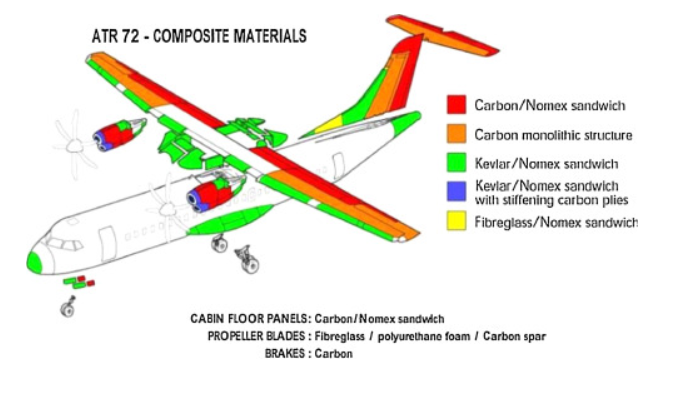
\includegraphics[width=0.75\textwidth]{Images-2-EstudoConceitual/figura1_composito_ATR72.png}
%     \caption{Uso restrito de material compósito no projeto do ATR 72.}
%     \label{fig:composito_atr72}
% \end{figure}

Atualmente, a indústria é dominada por projetos das décadas de 1980 e 1990, como o ATR 72, que possuem limitações arquitetônicas. Diante desse cenário de obsolescência, o desenvolvimento de uma aeronave inteiramente nova, ou "clean sheet", torna-se comercialmente viável e tecnicamente justificado, pois permite a redução substancial do peso vazio operacional através do uso extensivo de compósitos de última geração, por exemplo.

Além disso, um novo design pode viabilizar a integração nativa de sistemas de propulsão híbrida-elétrica e o preparo estrutural para o uso de 100\% de Combustível Sustentável de Aviação (SAF), garantindo conformidade operacional de longo prazo com as cada vez mais rigorosas regulações ambientais.

\subsubsection{O Ambiente Operacional Brasileiro}

No contexto doméstico, o Brasil apresenta um ambiente extremamente favorável, embora logisticamente desafiador, para a introdução dessa nova plataforma. Apesar de o país possuir milhares de municípios e mais de mil aeródromos registrados, apenas 157 localidades recebem voos comerciais regulares, evidenciando que a falta de capilaridade aérea decorre de barreiras de viabilidade econômica das aeronaves atuais e não apenas de limitações de infraestrutura física. 

Essa disparidade regional de acesso aéreo está detalhada espacialmente na Figura~\ref{fig:mapa_acesso} e quantificada na Tabela~\ref{tab:cobertura_aeroportuaria}, revelando  áreas desatendidas nas regiões Norte e Nordeste. 

\begin{figure}[H]
    \centering
    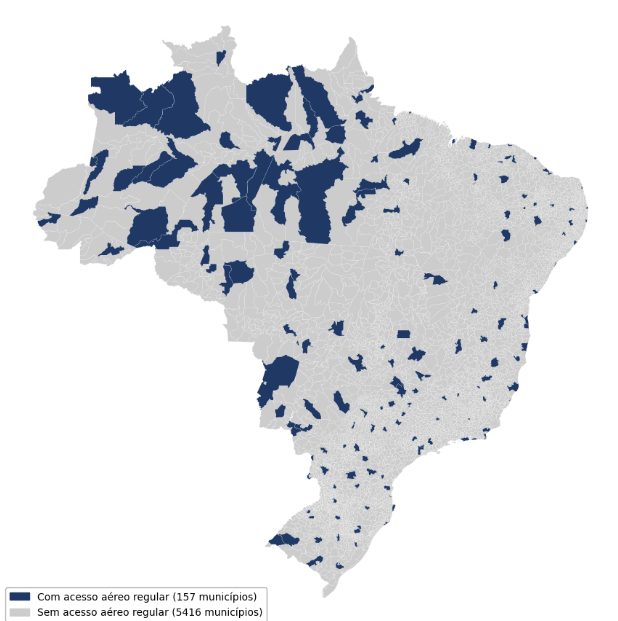
\includegraphics[width=0.6\textwidth]{Images-2-EstudoConceitual/figura2_mapa_coropletico.png}
    \caption{Municípios Brasileiros com e sem Acesso Aéreo Regular (2025).}
    \label{fig:mapa_acesso}
\end{figure}

\begin{table}[H]
\centering
\caption{Cobertura aeroportuária por macrorregião brasileira.}
\label{tab:cobertura_aeroportuaria}
\resizebox{\textwidth}{!}{
\begin{tabular}{l|c|c|c|c}
\hline
\textbf{Região} & \textbf{Municípios} & \textbf{Aeródromos Reg. (ANAC)} & \textbf{Municípios s/ Acesso Aéreo (est.)} & \textbf{Índice de Cobertura (\%)} \\ \hline
Norte & 450 & $\sim$105 & $\sim$375 & $\sim$23\% \\ \hline
Nordeste & 1.794 & $\sim$220 & $\sim$1.574 & $\sim$12\% \\ \hline
Centro-Oeste & 467 & $\sim$180 & $\sim$315 & $\sim$39\% \\ \hline
Sudeste & 1.668 & $\sim$410 & $\sim$1.258 & $\sim$25\% \\ \hline
Sul & 1.191 & $\sim$340 & $\sim$890 & $\sim$29\% \\ \hline
\textbf{Brasil (Total)} & \textbf{5.570} & \textbf{$\sim$1.255} & \textbf{$\sim$4.315} & \textbf{$\sim$22\%} \\ \hline
\end{tabular}
}
\end{table}

Para superar esses gargalos e destravar rotas inéditas, a capacidade do novo projeto de operar em pistas curtas, especificamente com decolagens em 4.200 pés e pousos em 3.000 pés, surge como um diferencial competitivo fundamental. 

O panorama atual do mercado interno é amplamente dominado pela Azul Linhas Aéreas, operadora que baseia suas estratégias em ligar o interior aos grandes centros, um cenário resumido na Tabela~\ref{tab:operadoras_regionais} e ilustrado pelas estatísticas de tráfego histórico de passageiros na Figura~\ref{fig:trafego_pax} e de participação de mercado na Figura~\ref{fig:market_share}. 

\begin{table}[H]
\centering
\caption{Principais operadoras de aviação regional no Brasil (2024).}
\label{tab:operadoras_regionais}
\resizebox{\textwidth}{!}{
\begin{tabular}{l|c|p{3.5cm}|p{3.5cm}|p{4.5cm}}
\hline
\textbf{Operadora} & \textbf{Destinos} & \textbf{Frota Regional} & \textbf{Mercado-Alvo} & \textbf{Observações Relevantes} \\ \hline
Azul Linhas Aéreas & $\sim$160 & ATR 72-600 (aprox. 39 un.) & Cidades médias e pequenas do interior & Maior malha regional do Brasil; opera $\sim$50\% de destinos exclusivos \\ \hline
VoePass (2024) & $\sim$40 & ATR 72-600 e ATR 42-500 & Interior de São Paulo, Sul e Centro Oeste & Possuía operações codeshare com LATAM; foco em rotas não atendidas por jatos \\ \hline
GOL / parceiras & $\sim$100 & Boeing 737 + parcerias & Hubs e alimentação via parceiros & Depende de operadoras menores para capilaridade; sem frota turboélice própria \\ \hline
\end{tabular}
}
\end{table}

\begin{figure}[H]
    \centering
    \begin{minipage}{0.48\textwidth}
        \centering
        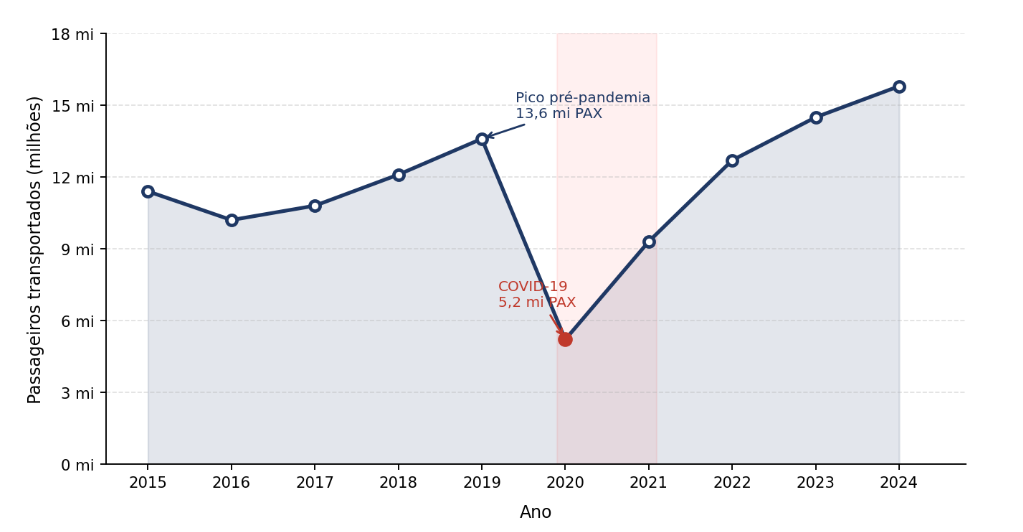
\includegraphics[width=\linewidth]{Images-2-EstudoConceitual/figura3_trafego.png}
        \caption{Tráfego histórico de passageiros na aviação regional brasileira.}
        \label{fig:trafego_pax}
    \end{minipage}
    \hfill
    \begin{minipage}{0.48\textwidth}
        \centering
        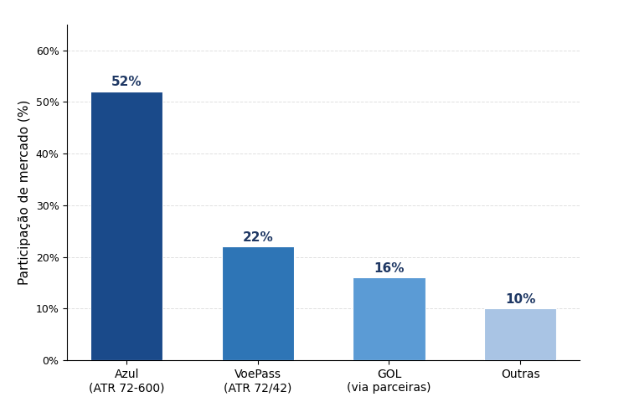
\includegraphics[width=\linewidth]{Images-2-EstudoConceitual/figura4_market_share.png}
        \caption{Participação de mercado das operadoras regionais (2024).}
        \label{fig:market_share}
    \end{minipage}
\end{figure}

Agravando a necessidade de inovação, a frota brasileira de turboélices em operação possui uma média de idade superior a 15 anos, o que catalisa a urgência de um iminente e expressivo ciclo de substituição.

\subsubsection{Conectividade e Demandas Internacionais}

A urgência por aeronaves regionais robustas e eficientes reverbera com igual intensidade em mercados internacionais estratégicos, ampliando o potencial de exportação do projeto. Na África, projeta-se um crescimento anual de tráfego aéreo de 5,1\% até 2043, concentrado em um continente onde a vasta maioria das cidades em desenvolvimento não dispõe de aeroportos com pistas pavimentadas compatíveis com jatos de médio porte. 

Similarmente, a macrorregião da Ásia-Pacífico lidera o ritmo de crescimento global do setor, impulsionada por políticas governamentais de interiorização do transporte na Índia (programa UDAN) e pela geografia arquipelágica da Indonésia, onde a expressiva economia de combustível dos turboélices é vital para viabilizar as ligações inter-ilhas. Em uma dinâmica diferente, mas complementar, o mercado maduro dos Estados Unidos demandará na próxima década a substituição direta de cerca de 800 jatos regionais defasados que alimentam seus complexos hubs, consolidando uma lógica de distribuição de tráfego que corrobora a utilidade universal de um avião regional moderno.

Essa convergência global de demandas e a necessidade latente de renovação de frota refletem-se de maneira contundente nas previsões para as próximas duas décadas. Como sumarizado na Tabela~\ref{tab:previsao_mercado} e ilustrado na Figura~\ref{fig:entregas_regionais}, a indústria aeronáutica projeta a entrega constante e volumosa de novas unidades para suprir a conectividade de curto e médio alcance.

\begin{table}[H]
\centering
\caption{Previsões de mercado para aeronaves regionais (50-90 assentos), 2024-2043.}
\label{tab:previsao_mercado}
\resizebox{\textwidth}{!}{
\begin{tabular}{l|c|c|p{4cm}|p{3.5cm}}
\hline
\textbf{Região / Segmento} & \textbf{Previsão de Entregas} & \textbf{Crescimento PAX} & \textbf{Déficit de Infraestrutura} & \textbf{Fonte} \\ \hline
América Latina (total) & $\sim$750 aeronaves & 4,5\% / ano & Poucas pistas pavimentadas & ATR Market Forecast 2024 \\ \hline
Brasil ($<$ 90 PAX) & $\sim$200-250 aeronaves & 3,8\% / ano & 4.300+ municípios sem acesso regular & ANAC / Embraer CMO 2024 \\ \hline
África Subsaariana & $\sim$450 aeronaves & 5,1\% / ano & Modal aéreo único em vastas regiões & IATA Industry Statistics 2024 \\ \hline
América do Norte & $\sim$800 aeronaves & 2,2\% / ano & Sistema hub-and-spoke maduro & FAA Aerospace Forecast 2024 \\ \hline
Ásia-Pacífico (incl. China) & $\sim$1.045 aeronaves & 5,2\% / ano & Geografia arquipelágica e cidades Tier 2/3 & ATR GMF / IATA \\ \hline
Oceania (incl. Austrália) & $\sim$125 aeronaves & 4,1\% / ano & Vastas distâncias e renovação de frota & Embraer CMO / Qantas \\ \hline
\end{tabular}
}
\end{table}

\begin{figure}[H]
    \centering
    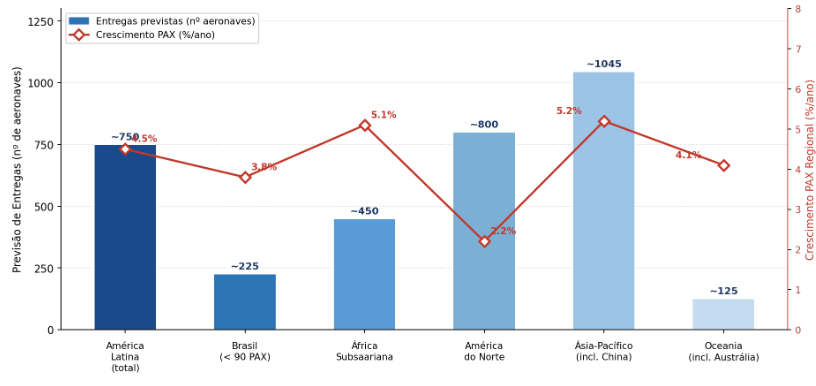
\includegraphics[width=0.85\textwidth]{Images-2-EstudoConceitual/figura6_entregas.png}
    \caption{Previsão global de entregas de aeronaves regionais (50-90 PAX) por região entre 2024 e 2043.}
    \label{fig:entregas_regionais}
\end{figure}

\subsection{Transporte de Cargas}

\subsubsection{Impacto do \textit{e-commerce}}

O setor que mais alavanca o transporte aéreo mundial de cargas é o e-commerce, com previsão de receita de mais de 6,4 trilhões de dólares para 2029, segundo dados da Statista Market Insights. No Brasil, a tendência de crescimento desse setor se mantém, sendo uma das maiores de todo o mundo, tal que uma pesquisa internacional da Insider Intelligence colocou o país entre os 10 com mais expectativa de crescimento do \textit{e-commerce} em 2022. Além disso, segundo a ABComm (Associação Brasileira de Comércio Eletrônico), a previsão para essa modalidade é um crescimento de 10\% ao ano até 2029, sem contar que, apenas para 2026, já prevê um número de 2 milhões de novos compradores \cite{gazetadopovo2026}.

Nesse sentido, gigantes do setor têm investido em malhas aéreas próprias para garantir diferenciais competitivos. A Amazon Air, por exemplo, registrou um crescimento de 102\% no número de voos diários entre 2020 e 2022. Paralelamente, o Mercado Livre (MELI AIR) expandiu sua frota visando reduzir o tempo de entrega nas capitais do Norte e Nordeste para apenas um dia. Esta tendência de crescimento nas entregas de compras pela internet reforça a necessidade de aeronaves regionais versáteis para essas operações \cite{gazetadopovo2026}.

\subsubsection{Matriz de Transporte Brasileira}

No cenário nacional, o modal aéreo apresenta uma participação de apenas 0,05\% do total de toneladas-quilômetros úteis (TKUs) movimentados, contrastando com os mais de 60\% do modal rodoviário. No entanto, esta baixa representatividade em volume bruto é paradoxal ao valor, já que o setor movimenta mercadorias de altíssimo valor agregado e urgência. Em 2022, o Brasil atingiu o seu recorde histórico de volume movimentado, totalizando 1,421 milhões de toneladas, com um aumento de 0,7\% em carga paga doméstica e 4,3\% em correios com relação ao ano anterior, conforme apresentado na Figura \ref{volume transportado de cargas}. Estes dados validam a existência de uma possível demanda por uma aeronave de médio porte, focada no transporte de bens nos quais a segurança e a rapidez justificam o custo do frete \cite{aeroincarga2026}.

\begin{figure} [H]
    \centering
    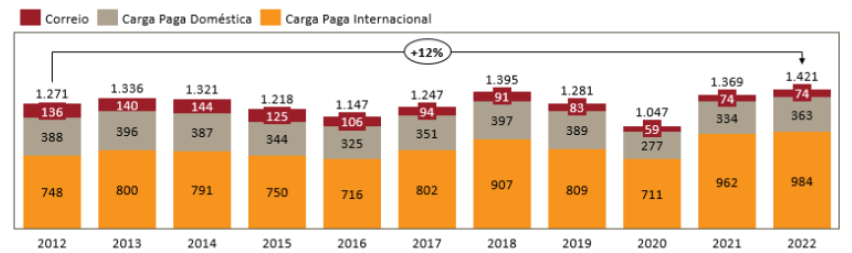
\includegraphics[width=0.9\linewidth]{images/Série histórica de transporte - Brasil.png}
    \caption{Série histórica do volume transportado de cargas pelo modal aéreo no Brasil, de 2012 a 2022 \cite{mercadolivre2022}.} 
    \label{volume transportado de cargas}
    
\end{figure}

Além disso, um ponto a ser levado em consideração são as principais rotas domésticas para transporte de cargas via modal aéreo no Brasil. Entre essas rotas, as quatro principais envolvem o aeroporto de Manaus (SBEG) e os aeroportos do estado de São Paulo – Guarulhos (SBGR) e Campinas (SBKP). O elevado fluxo aéreo entre estas duas regiões acontece pelo fato de Manaus ser uma região remota, com pouca estrutura rodoviária, porém que fabrica produtos de alto valor agregado por meio da Zona Franca de Manaus. Já o estado de São Paulo é o principal centro econômico do país, logo, consome grande parte das tecnologias que são produzidas na Zona Franca \cite{almeida2016}. 

Conforme retratado já na Figura \ref{fig:entregas_regionais} e explicado na seção anterior, o território brasileiro conta com uma deficiência em relação ao número de localidades com acesso aéreo regular. Dessa maneira, para poder utilizar os milhares de aeródromos registrados no Brasil para transportar cargas e, portanto, agilizar a logística no transporte de mercadorias em território nacional, há uma exigência de operação para pistas curtas de 4.200 ft (decolagem) e 3.000 ft (pouso).

Uma região altamente dependente dessa exigência técnica é o norte do país, de modo que, por possuir uma estrutura rodoviária precária, depende criticamente do modal aéreo. Alinhado ao que foi mencionado em relação ao fluxo concentrado entre Manaus (SBEG) e São Paulo (Guarulhos e Campinas), fica clara a necessidade de aeronaves operando nessa rota.

Além disso, a aviação regional constitui o elo vital entre estes grandes \textit{hubs} e cidades de médio porte. Estudos reforçam que pequenos aeroportos regionais impulsionam o desenvolvimento econômico local, mas enfrentam dificuldades para cobrir custos operacionais. Frotas eficientes com capacidades STOL (\textit{Short Take-Off and Landing}) e baixo custo operacional (DOC) são, portanto, a solução técnica para tornar estas rotas economicamente autossustentáveis.

\subsubsection{Conectividade e Demandas Internacionais}

Segundo a análise dos dados apresentados no \textit{Boeing World Air Cargo Forecast} \cite{boeing2024wacf}, projeta-se um cenário de resiliência e expansão para o setor de logística aérea nas próximas duas décadas, de modo que o mercado é caracterizado por um crescimento anual composto (CAGR) de 4,0\%, impulsionado pela digitalização do comércio global e pela reestruturação das cadeias de suprimentos. Além disso, um dos pontos mais relevantes para a análise de mercado é a composição da frota futura, estimada em 3.900 aeronaves até 2043.

No curto prazo, os dados de 2025 da pesquisa de \textit{Global Market Forecast} da Airbus \cite{airbus2025gmf} corroboram essa tendência de alta, registrando um crescimento mundial de 3,3\% no acumulado até agosto, apesar do desempenho regional heterogêneo, conforme apresentado na Figura \ref{fig:tráfego mundial de carga}.

\begin{figure} [H]
    \centering
    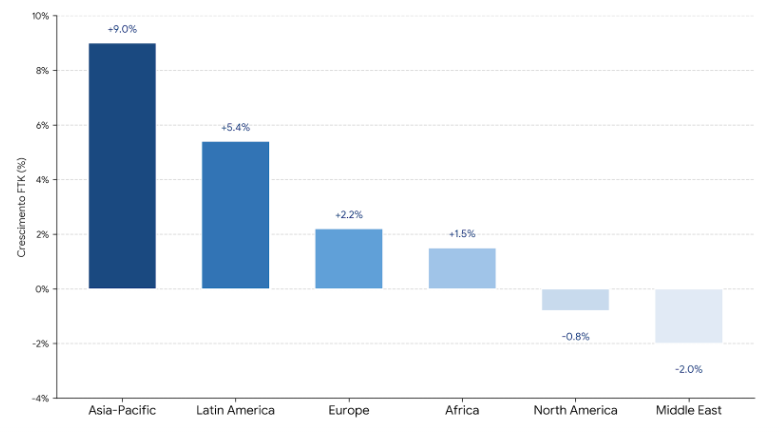
\includegraphics[width=0.8\linewidth]{images/Tráfego Mundial de Carga.png}
    \caption{Crescimento do tráfego de carga aérea por região (Jan - Ago 2025) \cite{airbus2025gmf}}
    \label{fig:tráfego mundial de carga}
\end{figure}

Por fim, é prevista uma consolidação de 25\% do \textit{share} para transportadoras expressas (como FedEx, DHL, UPS) até 2043, sendo esse um reflexo direto da irreversibilidade do \textit{e-commerce} transfronteiriço, o qual exige aeronaves com alta disponibilidade e ciclos rápidos, influenciando o \textit{design} de redes logísticas e a demanda por aeronaves de médio porte (\textit{narrow-body}) para alimentação de \textit{hubs} regionais. Nesse sentido, o mercado de carga aérea caminha para uma maior autonomia em relação ao transporte de passageiros. Para empresas do setor, o foco deve estar na eficiência operacional em mercados emergentes e na capacidade de execução de conversões de frota.

% --- SEÇÃO DE ESTUDO COMPARATIVO ---

\section{Estudos Comparativos}
\label{sec:estudoscomparativos}
O desenvolvimento do projeto conceitual é fundamentado em uma análise detalhada de aeronaves que operam no mesmo segmento ou que possuem características técnicas similares aos requisitos da seção~\ref{section:Requisitos}. Inicialmente, foram selecionadas 23 aeronaves, abrangendo uma ampla gama de modelos regionais, cargueiros e militares, com o intuito de estabelecer uma base para o esboço da geometria inicial.

A seleção baseou-se em parâmetros fundamentais como o Peso Máximo de Decolagem (MTOW), capacidade de passageiros, alcance e desempenho em pista \cite{medeiros2026}. A Tabela \ref{tab:comparativo_completo} apresenta os parâmetros básicos e essenciais dessas aeronaves, conforme levantamento realizado pelo grupo.


\begin{table}[H]
\centering
\caption{Levantamento abrangente de todas as aeronaves pesquisadas para análise estatística inicial.}
\label{tab:comparativo_completo}
\resizebox{\textwidth}{!}{%
\begin{tabular}{l|c|c|c|c|c|c}
\hline
\textbf{Modelo} & \textbf{Pax} & \textbf{MTOW [kgf]} & \textbf{$V_{cruise}$ [kt]} & \textbf{Alcance [nm]} & \textbf{Teto [ft]} & \textbf{Pista DE/PO [m]} \\ \hline
CASA C-295 & 71 & 21.000 & 260 & 3.040 & 30.000 & 978 / 789 \\ \hline
ATR 72-600 & 70-78 & 22.800 & 275 & 825 & 25.000 & 1.410 / 915 \\ \hline
Bombardier Dash 8 Q400 & 70-86 & 29.257 & 360 & 1.362 & 25.000 & 1.402 / 1.134 \\ \hline
Ilyushin Il-114-300 & 68 & 23.500 & 243 & 756 & 25.000 & 1.160 / 610 \\ \hline
NAMC YS-11 & 64 & 22.900 & 253 & 1.188 & 23.000 & 1.100 / 660 \\ \hline
BAe ATP & 64-70 & 22.930 & 268 & 985 & 25.000 & 1.460 / 1.130 \\ \hline
Saab 2000 & 50-58 & 22.999 & 370 & 1.549 & 31.000 & 1.355 / 1.200 \\ \hline
Antonov An-140-100 & 52 & 21.500 & 310 & 1.997 & 24.900 & 1.750 / 1.400 \\ \hline
Xian MA600 & 60 & 21.800 & 278 & 891 & 25.000 & 1.800 / 1.600 \\ \hline
Fokker 50 & 50 & 20.820 & 284 & 1.200 & 25.000 & 1.305 / 1.215 \\ \hline
Antonov An-26 & 40 & 24.000 & 237 & 1.300 & 24.600 & - / - \\ \hline
Leonardo C-27J Spartan & 62 & 32.500 & 325 & 3.160 & 30.000 & 690 / 390 \\ \hline
Short 360 "The Shed" & 36 & 12.292 & 212 & 915 & 20.000 & 1.158 / 853 \\ \hline
Mitsubishi SpaceJet (MRJ70) & 80 & 40.200 & 542 & 2.019 & 41.000 & 1.720 / 1.430 \\ \hline
Embraer ERJ 145 & 54 & 19.200 & 520 & 1.550 & 37.000 & 1.380 / 1.400 \\ \hline
Comac ARJ21-700 & 90 & 43.500 & 529 & 3.668 & 39.000 & 1.900 / 1.650 \\ \hline
Antonov An-148 & 92 & 43.700 & 470 & 1.275 & 40.000 & 1.685 / - \\ \hline
Transall C-160 & 93 & 51.000 & 320 & 4.780 & 27.000 & 730 / 550 \\ \hline
Embraer E190 & 104 & 47.790 & 547 & 2.850 & 41.000 & 1.267 / 1.244 \\ \hline
Saab 340F & 33-37 & 13.155 & 283 & 1.732 & 25.000 & 1.220 / 1.035 \\ \hline
Embraer EMB 110 & 18 & 5.788 & 236 & 1.118 & 21.000 & 380 / 400 \\ \hline
Cessna SkyCourier & 19 & 8.618 & 210 & 920 & 25.000 & 3.660 / 3.010 \\ \hline
Dornier Do 228 & 19 & 6.400 & 223 & 1.340 & 25.000 & 792 / 451 \\ \hline
\end{tabular}%
}
\end{table}

Após a avaliação, muitas aeronaves foram excluídas da análise por apresentarem divergências significativas em relação aos requisitos de missão estipulados para este projeto, a saber \cite{medeiros2026}:

\begin{itemize}
    \item \textbf{Propulsão e Regime de Velocidade:} Aeronaves equipadas com motores turbofan (ERJ 145, E190, SpaceJet, Antonov An-148) foram descartadas por operarem em velocidades de cruzeiro e altitudes muito superiores ao requisito de $260 \text{ kt}$ e $FL250$ \cite{medeiros2026}.
    \item \textbf{Porte e Capacidade:} Modelos como o Cessna SkyCourier, EMB 110 e Dornier 228, embora turboélices, possuem capacidade inferior a 20 passageiros, distanciando-se do requisito de 60 a 70 ocupantes \cite{medeiros2026}.
    \item \textbf{Missão e MTOW:} Aeronaves como o Transall C-160 e o Leonardo C-27J foram excluídas devido ao perfil de missão estritamente militar ou MTOW que excede o limite estabelecido de $50.000 \text{ lb}$ \cite{medeiros2026}.
\end{itemize}

Com base nestes critérios, as aeronaves selecionadas para compor a análise comparativa detalhada e fundamentar o Projeto Conceitual são: \textbf{ATR 72-600}, \textbf{CASA C-295}, \textbf{Ilyushin Il-114-300}, \textbf{BAe ATP}, \textbf{NAMC YS-11} e \textbf{Xian MA600}. Estas aeronaves representam os competidores diretos, conciliando a configuração turboélice, capacidade de passageiros e peso máximo de decolagem exigidos pelo projeto \cite{medeiros2026}. A Tabela \ref{tab:competidores_geometria} detalha os parâmetros geométricos e de desempenho dos modelos selecionados. 

\begin{table}[h!]
\centering
\caption{Parâmetros das aeronaves de referência selecionadas.}
\label{tab:competidores_geometria}
\resizebox{\textwidth}{!}{%
\begin{tabular}{l|c|c|c|c|c|c}
\hline
\textbf{Parâmetro} & \textbf{ATR 72-600} & \textbf{CASA C-295} & \textbf{Il-114-300} & \textbf{BAe ATP} & \textbf{NAMC YS-11} & \textbf{Xian MA600} \\ \hline
MTOW [kgf] & 22.800 & 21.000 & 23.500 & 23.700 & 22.900 & 21.800 \\ \hline
Área Alar [$m^2$] & 61,00 & 59,00 & 81,90 & 78,30 & 94,83 & 75,00 \\ \hline
Envergadura [m] & 27,05 & 25,81 & 29,87 & 30,63 & 32,00 & 29,20 \\ \hline
Nome do Motor & PW127M & PW127G & TV7-117ST-01 & PW126A & RR Dart Mk.542 & PW127J \\ \hline
Potência [shp] & 4.950 & 5290 & 5300 & 5306 & 5320 & 5762 \\ \hline
$V_{cruise}$ [kt] & 275 & 260 & 243 & 268 & 253 & 278 \\ \hline
$V_{stall}$ [kt] & 87 & 75-80 & 87 & 86 & 76 & 75 \\ \hline
Compr. Cabine [m] & 17,00 & 12,69 & 18,93 & 19,20 & 17,00 & 10,80 \\ \hline
Largura Cabine [m] & 2,57 & 2,70 & 2,64 & 2,48 & 2,70 & 2,70 \\ \hline
Altura Cabine [m] & 1,91 & 1,90 & 1,92 & 1,92 & 1,90 & 1,90 \\ \hline
Razão de Subida [ft/min] & 1.355 & 700 & 1000 & 1.000 & 1.220 & 1.500 \\ \hline
$N^\circ$ de Lugares & 70-78 & 71 & 68 & 64-70 & 64 & 60 \\ \hline
Alcance [nm] & 825 & 730 & 756 & 985 & 1.188 & 891 \\ \hline
Dist. Decolagem [m] & 1.410 & 978 & 1.160 & 1.460 & 1.100 & 1.800 \\ \hline
Dist. Pouso [m] & 915 & 789 & 610 & 1.130 & 660 & 1.600 \\ \hline
\end{tabular}%
}
\end{table}

\subsection{Configuração de Asa}

Para uma aeronave que deve cumprir missões de transporte regional de passageiros e de cargas a relativa baixa velocidade, a escolha de uma configuração de asa que permita bom desempenho em aerodinâmica e estabilidade, além da viabilidade operacional em aeroportos de menor infraestrutura é de suma importância.

Em primeira análise, a escolha entre uma asa alta, média ou baixa seria o primeiro passo, visto que cada uma por si só já trás características bem diferentes para os aspectos mencionados no parágrafo acima. De acordo com Anderson \cite{anderson1999}, uma asa alta favorece a capacidade operacional ao permitir que a fuselagem fique mais próxima do solo, permitindo cargas e descargas mais rápidas e com menos complexidade logística. Além disso, a asa alta tem um efeito estabilizante lateralmente muito forte, sendo, às vezes, necessário impor um diedro negativo (anedro) para aumentar a capacidade de rolamento da aeronave, por exemplo. Outro aspecto bastante positivo é que a asa alta fica longe do solo, permitindo motores maiores (no caso de \textit{turbofans}) e hélices maiores (no caso de motores convencionais ou turbohélices) sem a necessidade de uma estrutura que eleve a posição do motor (que aumentaria peso da aeronave).

Anderson \cite{anderson1999} explica também que asas médias são boas principalmente em questão de arrasto, visto que minimiza a interferência asa-fuselagem, porém pecam muito devido a necessidade de reforço estrutural na fuselagem e complicação para passagem de passageiros e/ou cargas.

Finalmente, asas baixas são boas em aproveitar o efeito solo (melhorando desempenho em pouso e decolagem). Porém, elas exigem que a fuselagem seja colocada numa altura maior do solo para permitir o posicionamento de motores/hélices. Além de que essa altura significa que o trem de pouso deve ser maior e consequentemente mais peso. \cite{anderson1999}

Tratando das características da asa em si, partimos de diversos parâmetros, como alongamento (\textit{Aspect Ratio - $AR$}), afilamento ($\lambda$), diedro ($\Gamma$), enflechamento no bordo de ataque ($\Lambda_{LE}$), a um quarto de corda ($\Lambda_{c/4}$), ângulo de incidência ($i_w$), entre outros.

O alongamento impacta em muitas características. Em geral, quanto maior o alongamento, melhor a eficiência ($L/D$) da asa, menor arrasto induzido, maior derivada $C_{L_\alpha}$, porém possui um amortecimento muito grande em relação ao rolamento, a asa é mais sucetível à flexão e a velocidade de \textit{flutter} é menor. Já asas pouco alongadas possuem ângulo de stall maior e menor peso estrutural. Porém possuem maior arrasto induzido, menor $C_{L_{max}}$ e propriedades aerodinâmicas de modo geral ruins para baixas velocidades \cite{gudmundsson2021}

Em relação ao afilamento (\textit{Taper Ratio}), a escolha normalmente está relacionada a um balanço entre característica de \textit{stall} e arrasto induzido. \cite{gudmundsson2021}

No que se trata do diedro, ele pode aumentar a estabilidade lateral da aeronave (diedro positivo) ou diminuir (anedro). Nesse sentido, o diedro positivo é  utilizado nas aeronaves comerciais para garantir voos mais estáveis e seguros, enquanto que o anedro é usado normalmente em projetos com asa alta ou com asas muito enflechadas, a fim de reduzir a força restauradora excessiva, preservando a manobrabilidade.

Já o ângulo de incidência da asa é, conforme Gudmundsson \cite{gudmundsson2021}, estabelecido primariamente para reduzir o arrasto em cruzeiro, pois permite que a asa opere no ângulo de ataque ótimo dessa fase enquanto a fuselagem se mantém alinhada ao escoamento (ângulo de ataque próximo de zero), evitando que esta gere arrasto adicional por operar fora de sua condição aerodinâmica ideal.

Por fim, o ângulo de enflechamento é normalmente utilizado por dois motivos principais: o posicionamento do centro de gravidade (CG) e a redução do arrasto de onda de choque em voos transônicos e supersônicos.


\subsection{Configuração das Empenagens}

A determinação da geometria das empenagem foi baseada, inicialmente, na análise dos coeficientes de volume de cauda. O coeficiente de volume de cauda horizontal é definido como:

\begin{equation}
V_{HT} = \frac{l_{HT} S_{HT}}{\bar{c} S}
\end{equation}

e o coeficiente de volume de cauda vertical como:

\begin{equation}
V_{VT} = \frac{l_{VT} S_{VT}}{b S}
\end{equation}

onde $l_{HT}$ e $l_{VT}$ são as distâncias entre o centro de gravidade da aeronave e os centros aerodinâmicos das respectivas superfícies, $S_{HT}$ e $S_{VT}$ são as áreas da empenagem horizontal e vertical, $\bar{c}$ é a corda média aerodinâmica da asa, $b$ é a envergadura da asa e $S$ é a área da asa \cite{anderson1999}. Esses coeficientes representam uma medida adimensional da capacidade das empenagens em gerar momentos estabilizantes, dentre outros.

No que diz respeito à configuração geométrica, existem diferentes arranjos possíveis para as empenagens, sendo os mais comuns a configuração convencional, a configuração em T e a configuração cruciforme. A configuração convencional, na qual a empenagem horizontal é posicionada na base da empenagem vertical (ou diretamente na fuselagem), é a mais utilizada, estando presente na maioria das aeronaves devido à  simplicidade estrutural, menor peso e bom compromisso entre estabilidade e controle.

Já configuração em T posiciona a empenagem horizontal no topo da empenagem vertical, trazendo algumas vantagens aerodinâmicas, como a redução da interferência com a esteira da asa. No entanto, apresenta desvantagens estruturais significativas, exigindo reforços pesados na empenagem vertical.

Já a configuração cruciforme representa um compromisso entre as duas anteriores, posicionando a empenagem horizontal em uma posição intermediária na empenagem vertical, buscando equilibrar os benefícios aerodinâmicos e estruturais \cite{anderson1999}.

O posicionamento longitudinal das empenagens resulta de um compromisso entre ganho de autoridade e aumento de peso estrutural. Em geral, busca-se posicionar a cauda mais afastada do centro de gravidade para aumentar o braço de alavanca ($l_{HT}$ e $l_{VT}$), reduzindo a área necessária das superfícies para um mesmo efeito estabilizante. Entretanto, esse aumento do braço também exige uma fuselagem estruturalmente mais robusta e, consequentemente, mais pesada, devendo ambos os efeitos ser balanceados no projeto \cite{anderson1999}.


\subsection{Configuração de Cabine}

O dimensionamento interno da fuselagem é tradicionalmente realizado por meio de um processo de dentro para fora, no qual a cabine de passageiros e o compartimento de carga determinam a geometria das seções transversal e longitudinal, posteriormente refinada com base em critérios aerodinâmicos externos \cite{raymer2018}. Para esta aeronave, projetada para acomodar entre 60 e 70 passageiros, a prioridade é atender aos requisitos de conforto, ergonomia e flexibilidade de missão.


A cabine adotará uma configuração de 4 assentos por fileira (2+2), separados por um corredor central, o que representa o padrão da indústria para turboélices regionais deste porte. Além disso, o projeto prevê trilhos estruturais no piso para permitir a rápida conversão entre a configuração de passageiros e o transporte de carga utilizando ULDs, contêineres e pallets padronizados. A porta principal de carga será dimensionada para permitir a passagem desses dispositivos, respeitando as normas internacionais para operações logísticas.

A fim de balizar as dimensões principais da fuselagem (comprimento, largura e altura interna), realizou-se uma análise estatística dos seis concorrentes diretos aprovados na filtragem do Projeto Conceitual. Os resultados deste comparativo estão expressos nas Figuras \ref{fig:bar_comp_cabine}, \ref{fig:bar_largura_cabine} e \ref{fig:bar_altura_cabine}.

\begin{figure}[H]
    \centering
    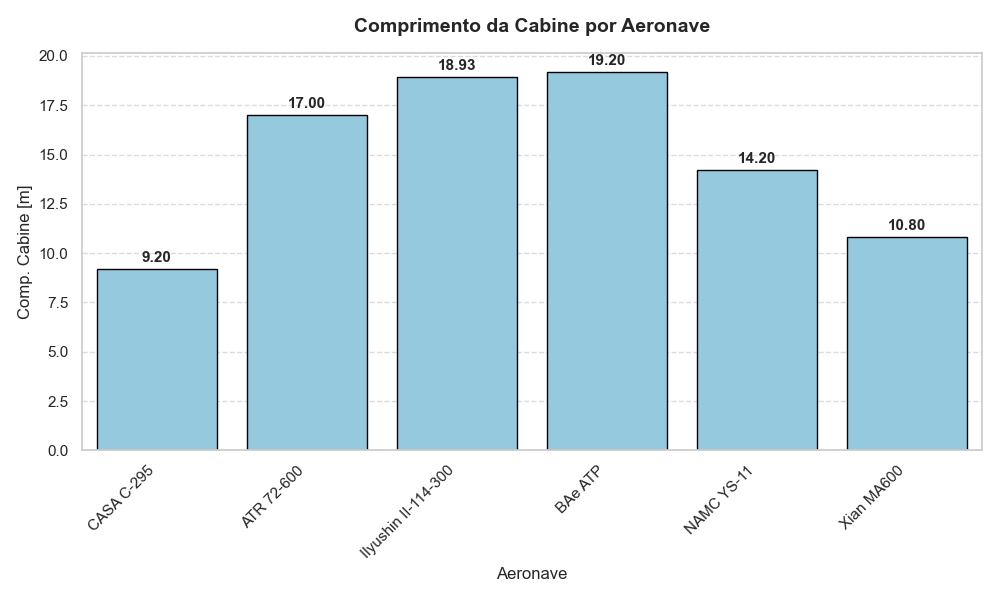
\includegraphics[width=0.75\linewidth]{Images-2-EstudoConceitual/Comp_cabine.png} % Ajuste o caminho se necessário
    \caption{Comparativo do comprimento da cabine entre as aeronaves de referência.}
    \label{fig:bar_comp_cabine}
\end{figure}

\begin{figure}[H]
    \centering
    \begin{minipage}{0.48\textwidth}
        \centering
        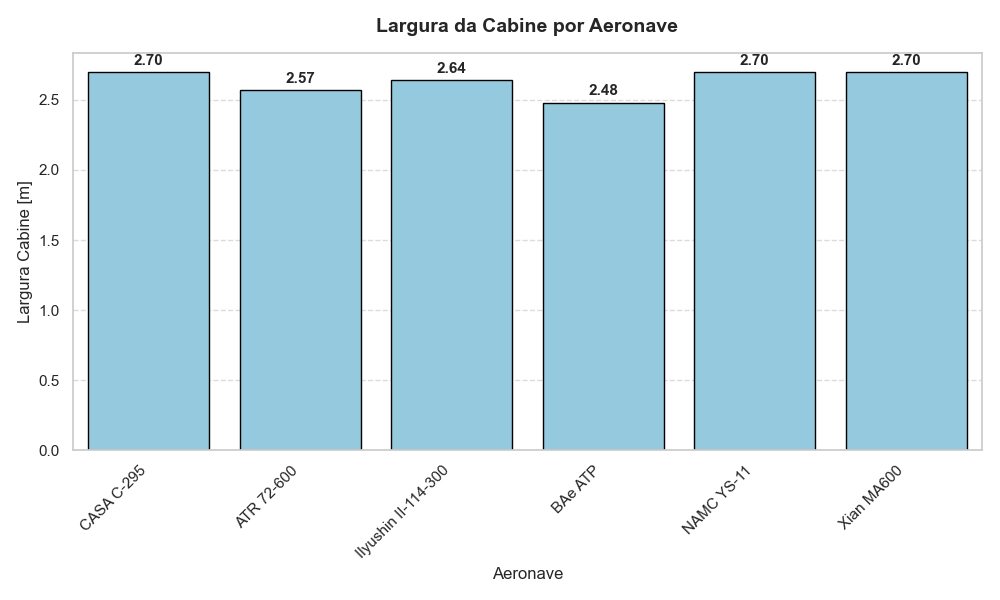
\includegraphics[width=\linewidth]{Images-2-EstudoConceitual/Larg_cabine.png} % Ajuste o caminho se necessário
        \caption{Largura interna da cabine.}
        \label{fig:bar_largura_cabine}
    \end{minipage}
    \hfill
    \begin{minipage}{0.48\textwidth}
        \centering
        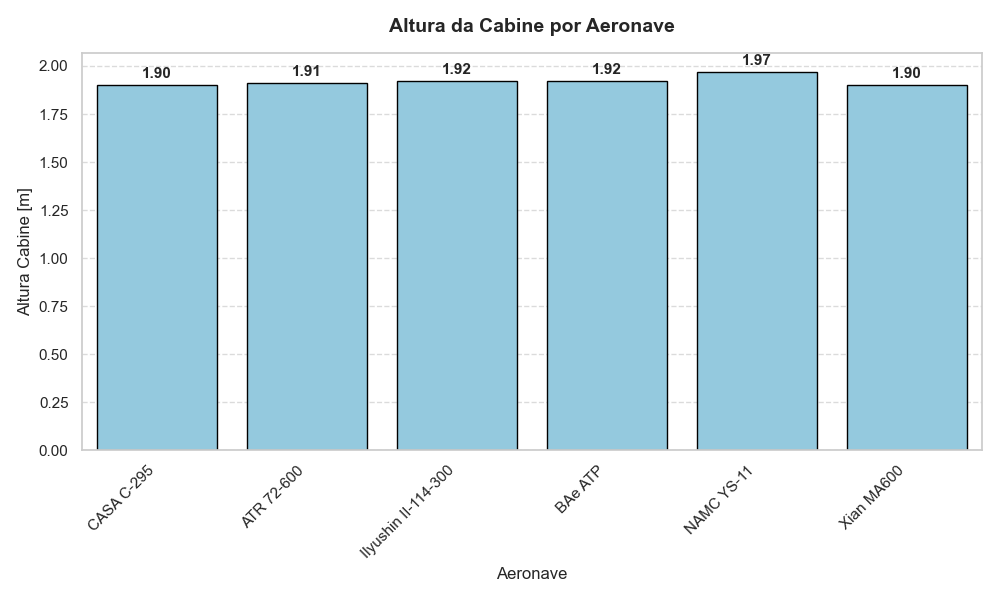
\includegraphics[width=\linewidth]{Images-2-EstudoConceitual/Alt_cabine.png} % Ajuste o caminho se necessário
        \caption{Altura interna da cabine.}
        \label{fig:bar_altura_cabine}
    \end{minipage}
\end{figure}

A análise da Figura \ref{fig:bar_comp_cabine} revela uma variância significativa no comprimento da cabine em função do perfil da missão. O modelo CASA C-295 apresenta um valor nitidamente inferior (9,20 m) por ser uma aeronave de origem militar. Em contrapartida, as aeronaves dedicadas primariamente ao transporte civil de passageiros (como o ATR 72, Il-114 e YS-11) agrupam-se na faixa de 14,00 m a 19,00 m. Para acomodar as fileiras de assentos com o \textit{pitch} (espaçamento) padrão da classe, adicionando espaço para \textit{galleys} (copa) e lavatórios, o Projeto Conceitual adotará um comprimento de cabine em torno de 17,00 m.

Quanto à seção transversal, as Figuras \ref{fig:bar_largura_cabine} e \ref{fig:bar_altura_cabine} demonstram uma forte padronização de mercado. A altura interna varia em uma margem muito estreita (entre 1,90 m e 1,97 m), dimensão estritamente necessária para garantir a ergonomia e permitir que um passageiro adulto do percentil 95 caminhe ereto pelo corredor. 

A largura interna concentra-se entre 2,48 m e 2,70 m, o que é suficiente para acomodar confortavelmente dois assentos duplos (com largura média de 1,00 m a 1,05 m cada par) e um corredor central normativo de no mínimo 0,45 m. 

\subsection{Configuração de Propulsão}

A definição da configuração de propulsão da aeronave foi baseada nos estudos comparativos apresentados. Para a aeronave em estudo, cuja velocidade de cruzeiro máxima é de aproximadamente 260 kt, observa-se que este regime de voo está abaixo da faixa em que motores do tipo turbofan apresentam maior eficiência. Motores turbofan são mais adequados para aeronaves que operam em velocidades mais elevadas e maiores altitudes, nas quais os ganhos associados à propulsão a jato se tornam mais significativos. Em contrapartida, em regimes de baixa a média velocidade, típicos da aviação regional, os motores turboélice apresentam melhor eficiência propulsiva, resultando em menor consumo de combustível para a mesma missão.

Quanto aos motores alternativos, eles apresentam três limitações intrínsecas que dificultam o uso em aeronaves de maior porte. A relação potência-peso é desfavorável, pois o aumento de potência exige mais cilindrada e por consequência um aumento grande de massa. A eficiência cai com a altitude, já que motores aspirados dependem da densidade do ar admitido, perdendo potência conforme a aeronave sobe, limitação que a turbina, com sua razão de compressão interna, não sofre na mesma intensidade, esse problema poderia ser parcialmente resolvido com turbocompressores ou turbonormalizadores, mas no fim existirá ainda mais aumento de peso. Por fim, a vida útil entre revisões é menor, consequência direta da maior quantidade de peças móveis sujeitas a desgaste e fadiga (válvulas, anéis, ignição), o que aumenta a frequência de manutenção em comparação ao turboélice.

Além da eficiência em cruzeiro, os motores turboélice apresentam vantagens operacionais importantes para o perfil da aeronave proposta. Entre elas, destacam-se a melhor performance em decolagens e pousos em pistas curtas, maior eficiência em altitudes moderadas e maior robustez para operações em aeroportos com infraestrutura limitada. Tais características são particularmente relevantes considerando os requisitos de operação da aeronave, que incluem pistas de comprimento reduzido e voos regionais de curta e média distância.

Outro fator determinante é o custo operacional. Motores turboélice, em geral, apresentam menor consumo específico de combustível em regimes subsônicos baixos e, apesar de um custo mais elevado no ciclo de manutenção, são mais baratos. 

No que se refere à redundância e segurança operacional, a adoção de uma configuração bimotor é considerada essencial. Essa configuração permite que a aeronave mantenha capacidade de voo segura mesmo em caso de falha de um dos motores, atendendo aos requisitos de certificação e ampliando a flexibilidade operacional, especialmente em rotas que envolvem regiões com infraestrutura limitada. 

Dessa forma, a configuração bimotor turboélice foi selecionada como a mais adequada para a aeronave em estudo, proporcionando um equilíbrio entre eficiência em cruzeiro, desempenho em operações de pista curta, custos operacionais e segurança, atendendo de forma consistente às exigências das missões de transporte regional de passageiros e carga.

\subsection{Configuração do Trem de Pouso}

Adotou-se a geometria de trem de pouso triciclo retrátil, configuração que representa o padrão da indústria para aeronaves comerciais modernas por garantir estabilidade direcional superior durante o táxi e facilitar as operações de pouso e decolagem, além de ser o caso de todas as aeronaves mencionadas na tabela \ref{tab:competidores_geometria}.

Para a absorção de impactos, a engenharia consolidou arquiteturas distintas. Os amortecedores óleo-pneumáticos com tesoura de torção, ilustrados na Figura \ref{fig:oleopneumatic}, utilizam a compressibilidade do nitrogênio como mola pneumática para suportar o peso estático e o óleo hidráulico para dissipar a energia do impacto através de um orifício medidor. Outra solução complexa é o braço arrastado (\textit{trailing link}), apresentado na Figura \ref{fig:TrailingArm}, que utiliza um braço articulado atuando como alavanca para proporcionar uma compressão mais progressiva do amortecedor, sendo excepcionalmente eficaz na absorção de cargas verticais e horizontais em pistas irregulares ou pousos de alta energia.

Embora soluções simplificadas como a lâmina de aço mola ou cordas elásticas (\textit{bungee cords}) sejam elegantes pela baixa complexidade, elas apresentam amortecimento limitado e propensão a saltos (\textit{bounces}) em pousos mais bruscos. Tais arquiteturas são restritas a aeronaves leves ou de treinamento e não são viáveis para a classe de peso de 50.000 lb deste projeto. 

Devido à configuração de asa alta, o trem de pouso principal será recolhido em carenagens laterais fixadas na fuselagem. Esta escolha preserva a integridade estrutural da asa e permite que o piso da aeronave permaneça baixo e nivelado, otimizando o carregamento de carga e o acesso de passageiros. Os amortecedores selecionados serão do tipo óleo-pneumático, dimensionados para suportar as cargas operacionais de uma aeronave regional de médio porte.

\begin{figure}[H]
    \centering
    % Primeira figura - Óleo-Pneumático
    \begin{minipage}{0.3\textwidth}
        \centering
        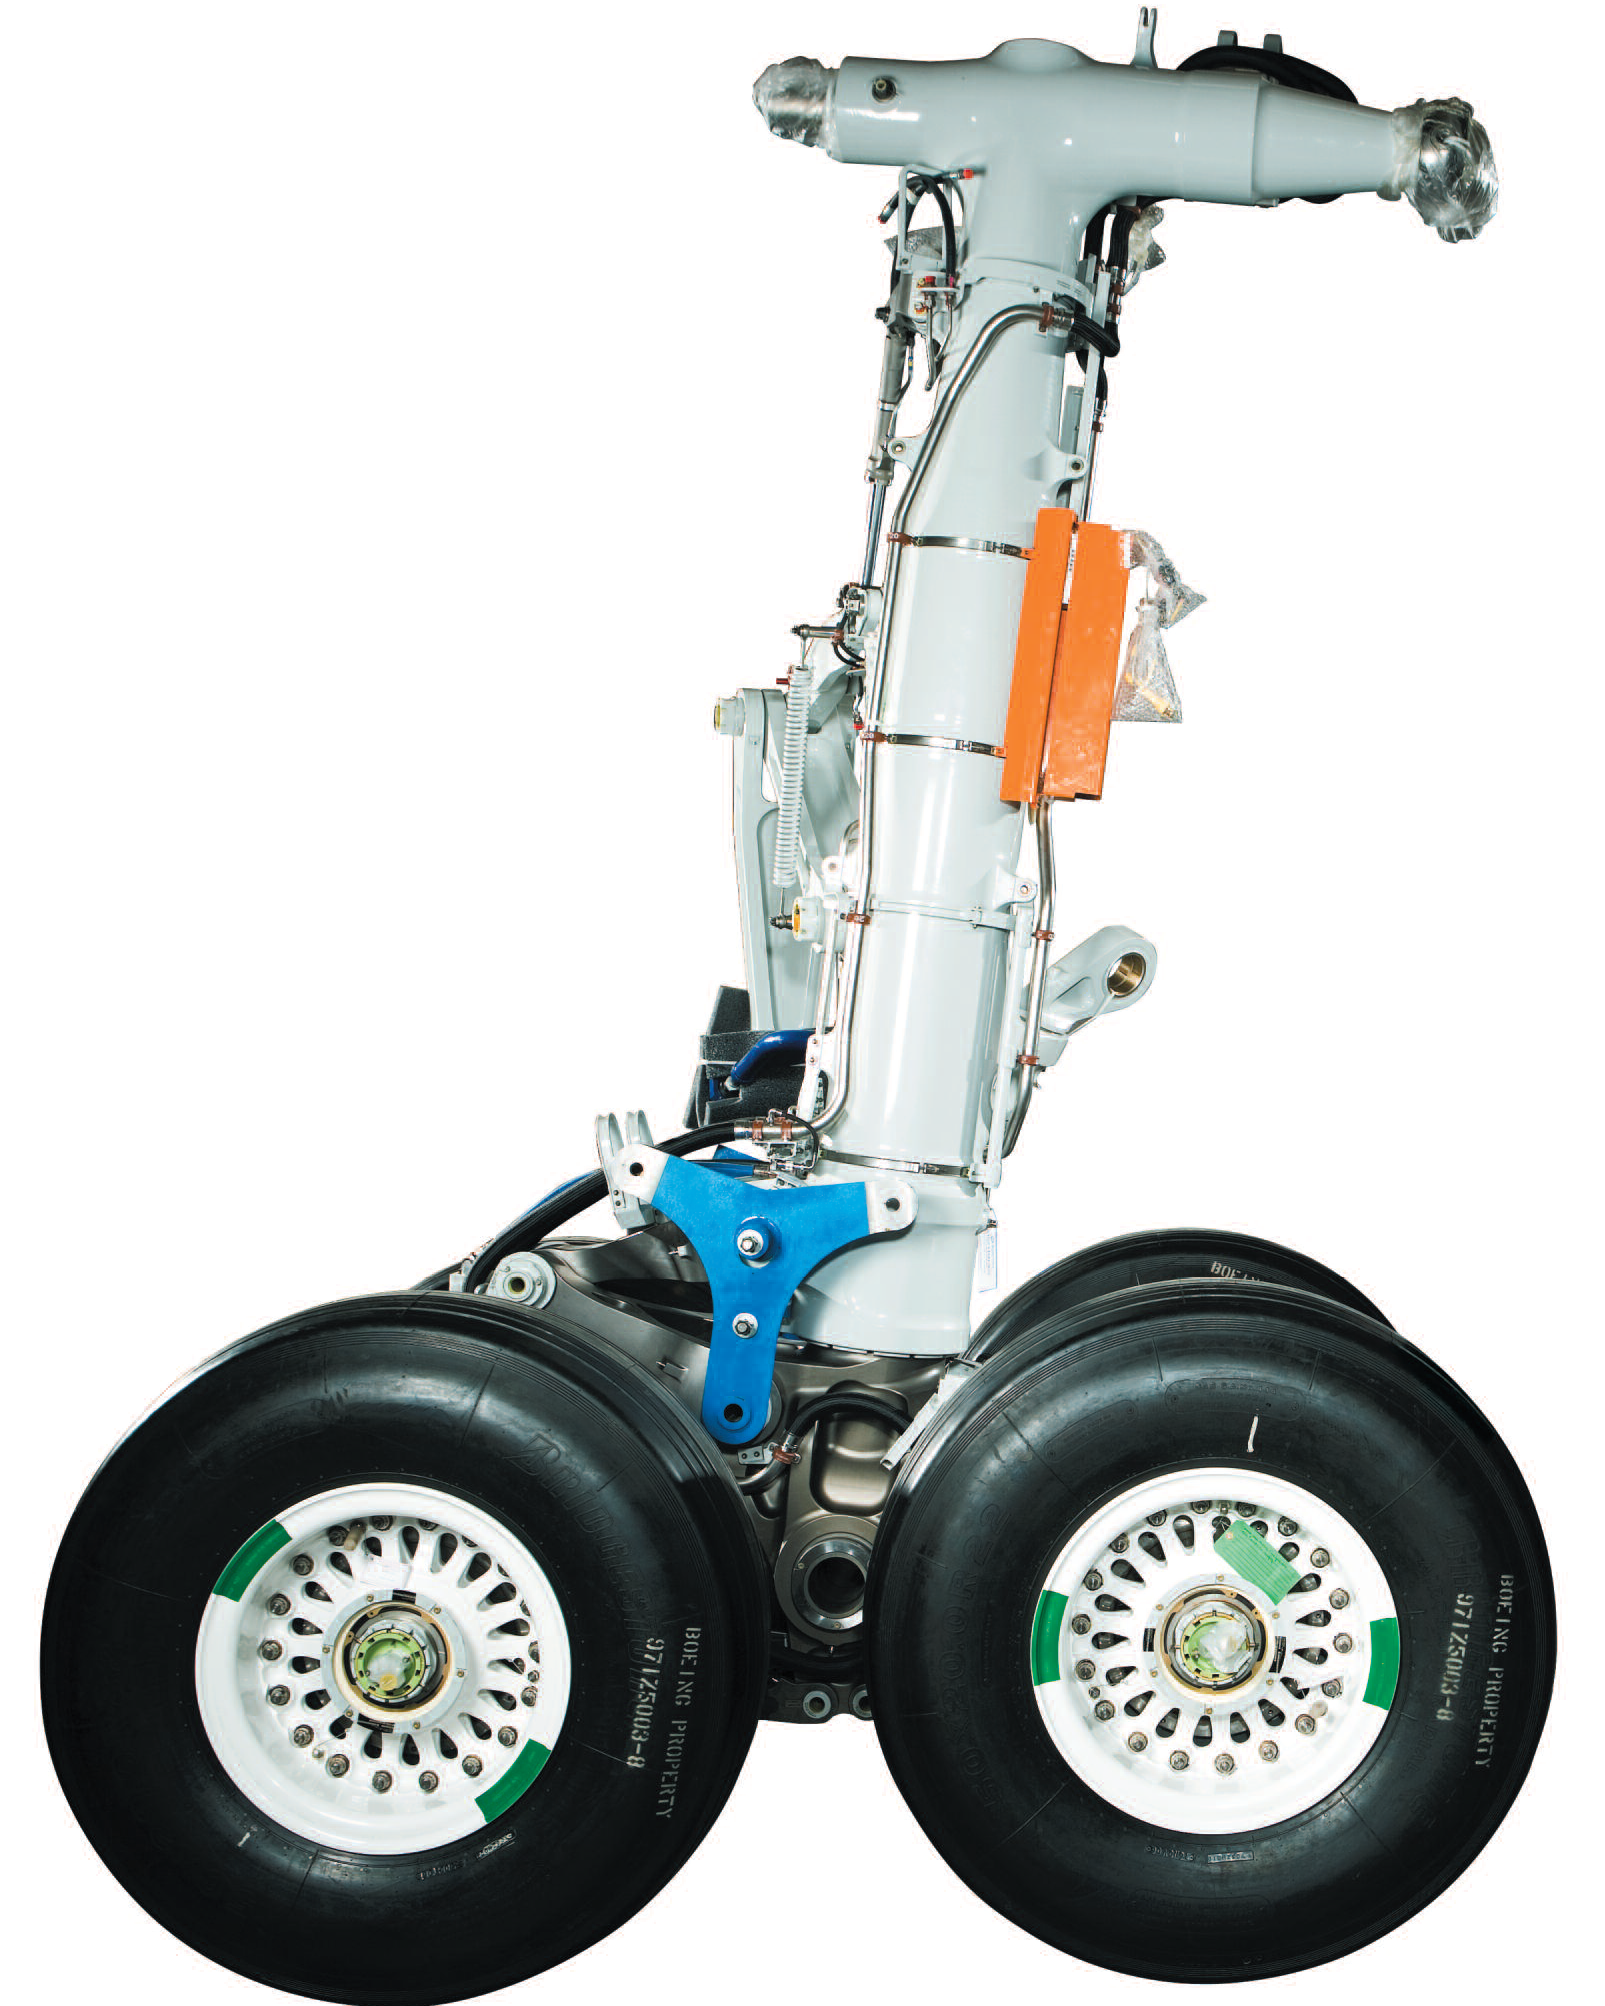
\includegraphics[width=\linewidth]{Images-2-EstudoConceitual/oleo_pneumatic.png} 
        \caption{Amortecedor óleo-pneumático \cite{globalspec_oleo}.}
        \label{fig:oleopneumatic}
    \end{minipage}
    \hfill
    % Segunda figura - Trailing Link
    \begin{minipage}{0.3\textwidth}
        \centering
        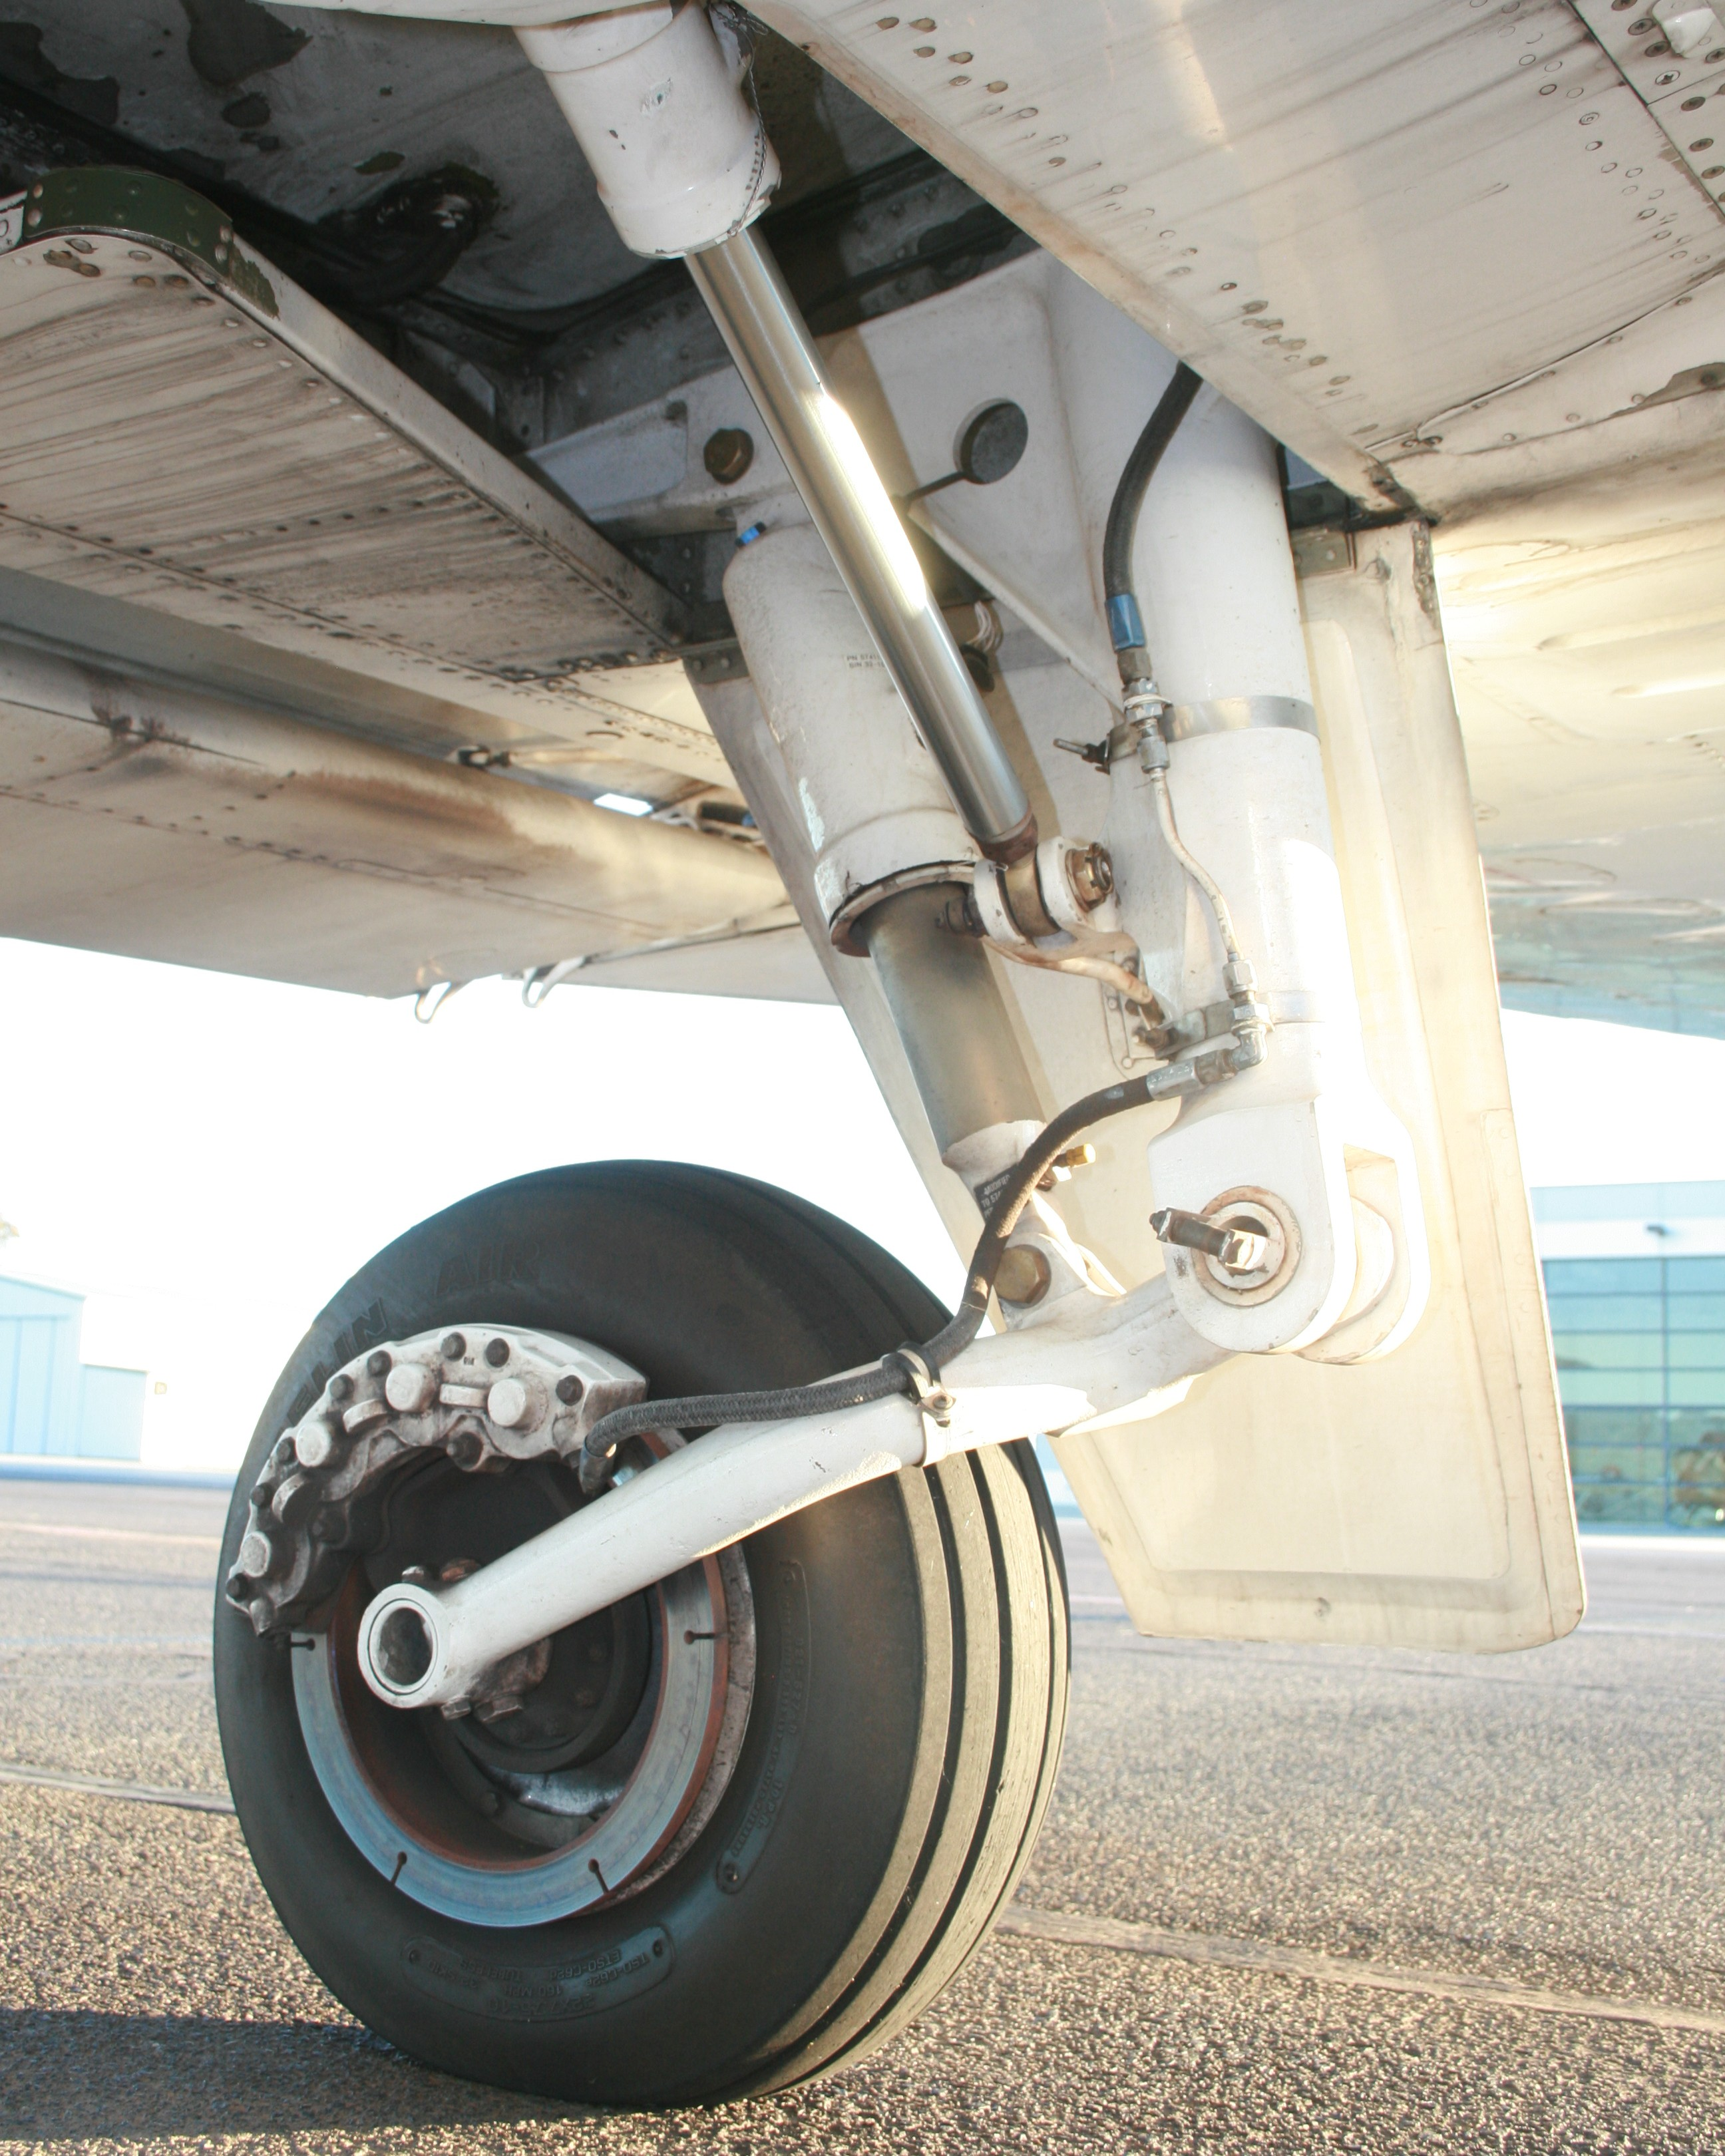
\includegraphics[width=\linewidth]{Images-2-EstudoConceitual/trailing_link.jpg} 
        \caption{Arquitetura de trem de pouso do tipo \textit{Trailing Link}\cite{wikimedia_trailing}.}
        \label{fig:TrailingArm}
    \end{minipage}
\end{figure}

Quanto ao funcionamento de amortecedores de trens de pouso óleo-pneumáticos, existem duas soluções principais: amortecedores com placa e metering pin ou com metering tube. O primeiro tipo, ilustrado na Figura \ref{fig:meteringpin}, se destaca por utilizar placas com orifício atravessadas por um pino de seção variável em um formato cônico, de forma que, quanto maior for a contração do trem de pouso após o contato completo com o solo, menor será a folga entre o orifício e o metering pin, aumentando a fricção do fluido com a estrutura e, consequentemente, dispersando a energia absorvida na forma de calor. Já os sistemas com metering tube, referenciados na Figura \ref{fig:meteringtube}, utilizam um tubo vazado com diversos orifícios, através dos quais o fluido é forçado durante a contração do trem, com o mesmo objetivo de rejeição de energia na forma de calor, sendo uma solução mais simplificada. 

Assim, para este projeto, a solução adotada será a do sistema com metering pin, uma vez que este é o sistema mais comumente usado, além de possuir a vantagem de permitir um ajuste e controle da dissipação de energia mais refinado quando comparado aos amortecedores com metering tube.

\begin{figure}[H]
    \centering
    % Primeira figura - metering pin
    \begin{minipage}{0.5\textwidth}
        \centering
        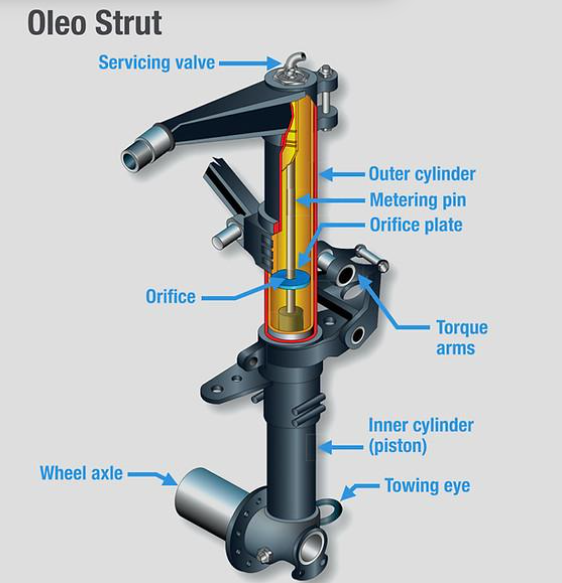
\includegraphics[width=\linewidth]{images/metering pin.png} 
        \caption{Amortecedor com metering pin \cite{meteringpin}.}
        \label{fig:meteringpin}
    \end{minipage}
    \hfill
    % Segunda figura - metering tube
    \begin{minipage}{0.3\textwidth}
        \centering
        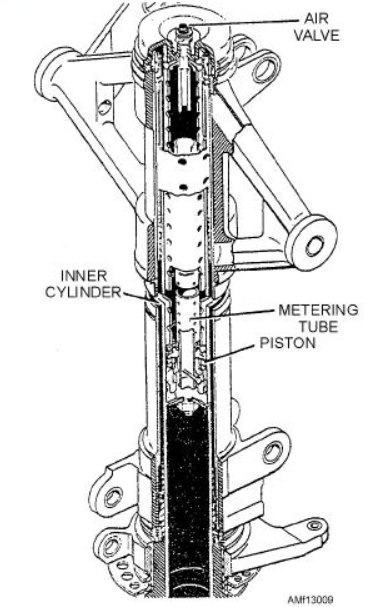
\includegraphics[width=\linewidth]{images/metering tube.png} 
        \caption{Amortecedor com metering tube \cite{meteringtube}.}
        \label{fig:meteringtube}
    \end{minipage}
\end{figure}


\section{Verificação de Requisitos e Tendências de Mercado}

Antes de consolidar as características gerais do protótipo e iniciar o projeto conceitual, é imprescindível confrontar os requisitos de missão estipulados com os dados reais de desempenho e peso dos concorrentes selecionados. Essa correlação gráfica permite validar se as metas do projeto são fisicamente factíveis e identificar os desafios tecnológicos que deverão ser superados.

A Figura \ref{fig:teto_v_cruzeiro} correlaciona o Teto de Operação com a Velocidade de Cruzeiro ($V_{cruise}$). O requisito do projeto exige uma operação a 260 kt e teto de 25.000 ft. Nota-se que o requisito encontra-se perfeitamente centralizado no envelope operacional da classe. Aeronaves como o BAe ATP e o ATR 72-600 operam com velocidades levemente superiores, enquanto o CASA C-295 apresenta um teto de serviço substancialmente maior (30.000 ft) devido à sua vocação tática. O ponto de projeto estipulado é, portanto, conservador e perfeitamente atingível com a tecnologia turboélice atual.

\begin{figure}[H]
    \centering
    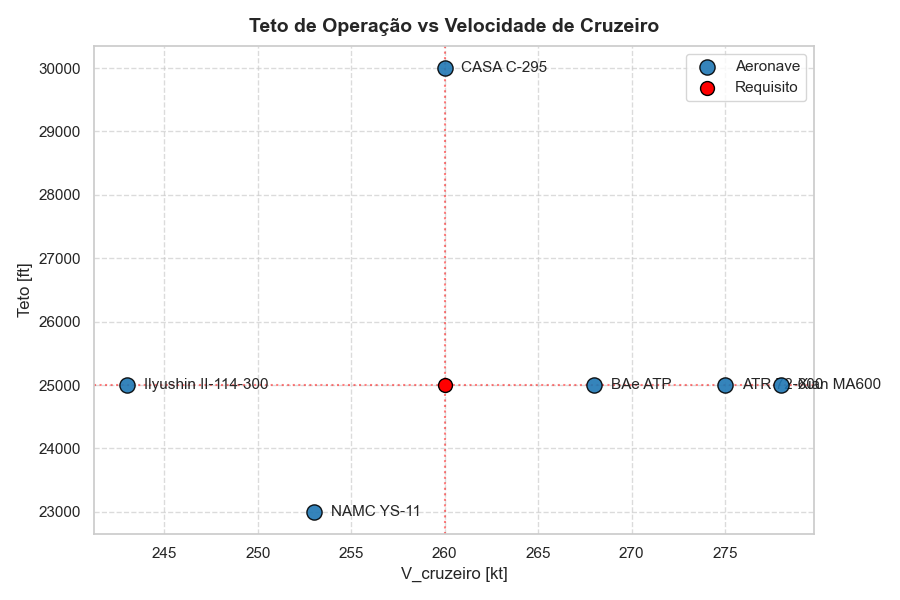
\includegraphics[width=0.7\linewidth]{Images-2-EstudoConceitual/teto_x_v_cruzeiro.png}
    \caption{Correlação entre Teto de Operação e Velocidade de Cruzeiro das aeronaves de referência em relação ao requisito de projeto.}
    \label{fig:teto_v_cruzeiro}
\end{figure}

Do ponto de vista de estimativa de massas, a Figura \ref{fig:pv_mtow} ilustra a relação entre o Peso Vazio (PV) e o Peso Máximo de Decolagem (MTOW). Observa-se uma tendência linear de crescimento do peso vazio em função do MTOW, característica típica demonstrada pelas formulações empíricas de Raymer \cite{raymer2018} e Roskam. O MTOW alvo do projeto encontra-se na faixa de 22.500 kgf. A dispersão dos dados mostra que aeronaves otimizadas para passageiros (como o ATR 72-600) conseguem manter um peso vazio estrutural mais baixo em relação ao MTOW do que aeronaves mais antigas ou adaptadas (como o YS-11), indicando a importância do uso de materiais compostos e ligas avançadas para o Projeto Conceitual.

\begin{figure}[H]
    \centering
    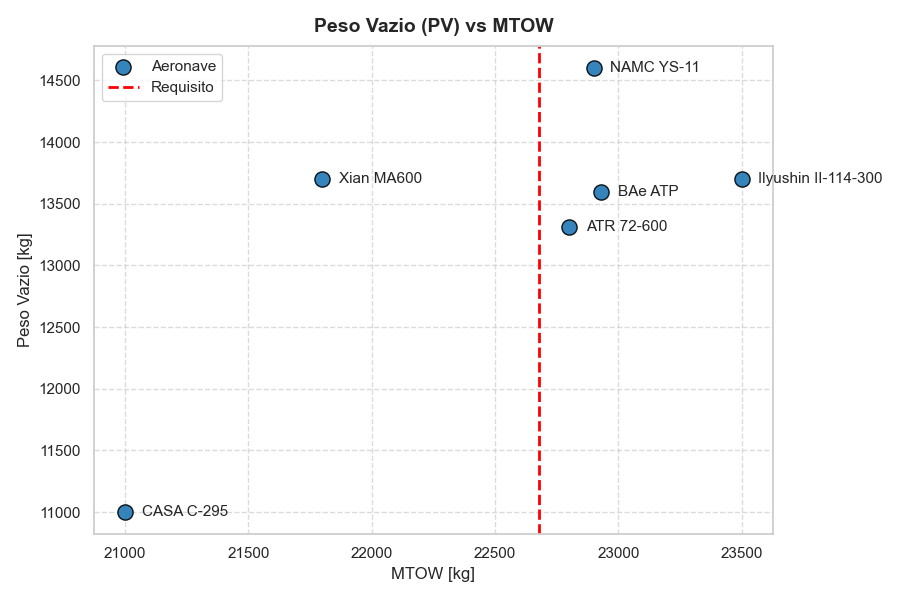
\includegraphics[width=0.7\linewidth]{Images-2-EstudoConceitual/pv_x_mtow.png}
    \caption{Tendência de Peso Vazio em função do Peso Máximo de Decolagem (MTOW).}
    \label{fig:pv_mtow}
\end{figure}

Por fim, o desempenho em pista é avaliado nas Figuras \ref{fig:pouso_mtow} e \ref{fig:decolagem_mtow}. O requisito de projeto dita um comprimento máximo de pista de aproximadamente 1.280 m para ambas as operações. 

\begin{figure}[H]
    \centering
    \begin{minipage}{0.48\textwidth}
        \centering
        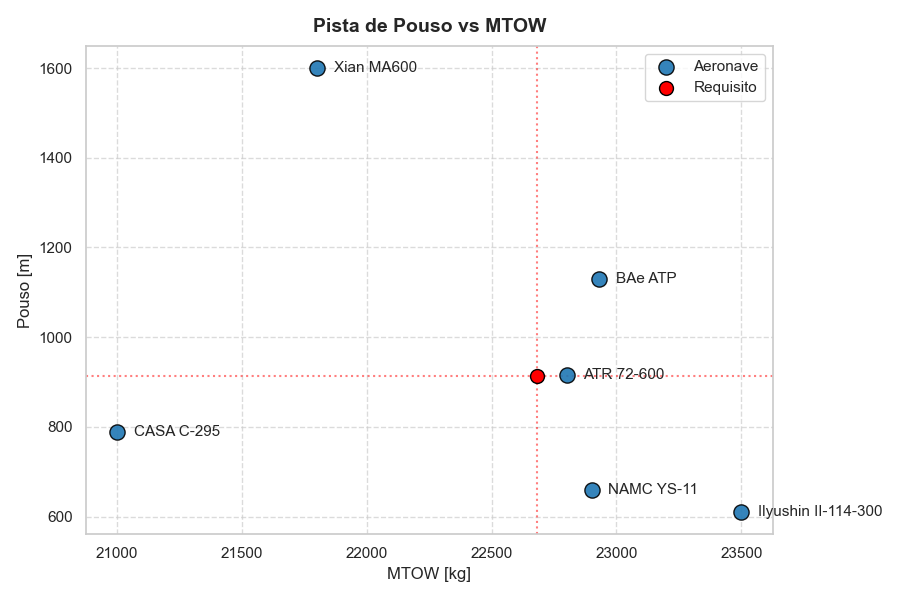
\includegraphics[width=\linewidth]{Images-2-EstudoConceitual/pouso_x_MTOW.png}
        \caption{Distância de Pouso vs MTOW.}
        \label{fig:pouso_mtow}
    \end{minipage}
    \hfill
    \begin{minipage}{0.48\textwidth}
        \centering
        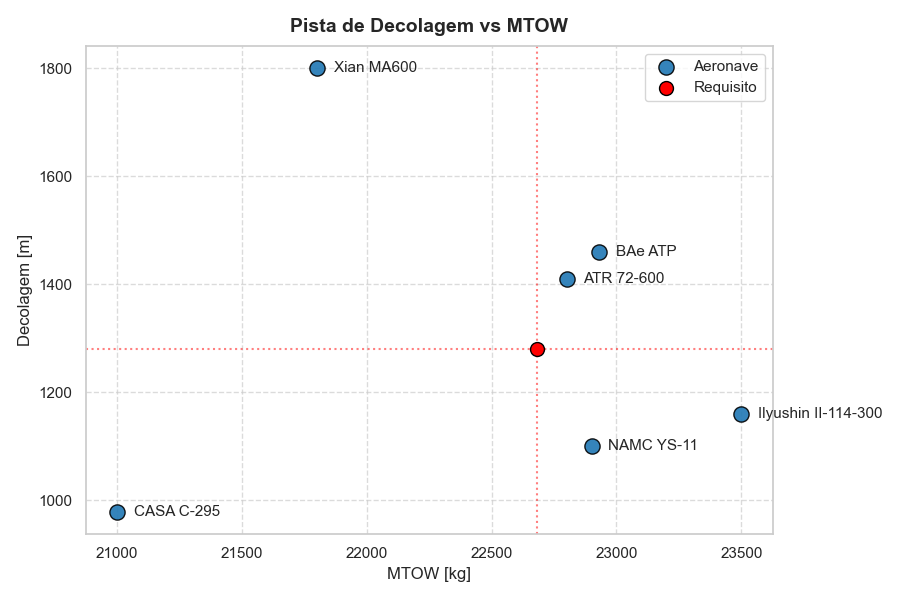
\includegraphics[width=\linewidth]{Images-2-EstudoConceitual/decolagem_x_mtow.png}
        \caption{Distância de Decolagem vs MTOW.}
        \label{fig:decolagem_mtow}
    \end{minipage}
\end{figure}

Para o pouso (Figura \ref{fig:pouso_mtow}), o requisito é atendido com certa margem pela maioria das aeronaves. No entanto, a decolagem (Figura \ref{fig:decolagem_mtow}) revela-se como a fase crítica limitante do projeto. Modelos como o ATR 72-600, Xian MA600 e BAe ATP ultrapassam a restrição de decolagem, evidenciando que, para atingir o MTOW de projeto e ainda operar em pistas curtas, o Projeto Conceitual precisará focar rigorosamente em um sistema hipersustentador eficiente (elevado $C_{L_{max}}$ de decolagem) e em uma baixa carga alar ($W/S$).

\section{Delimitação Geral do Protótipo}

Após a análise comparativa detalhada e a avaliação das características predominantes entre os competidores diretos, a Tabela \ref{tab:delimitacao_prototipo} sintetiza as configurações selecionadas para o desenvolvimento do Projeto Conceitual da aeronave.

\begin{table}[h!]
\centering
\caption{Características desejadas para os componentes da aeronave.}
\label{tab:delimitacao_prototipo}
\vspace{0.2cm} % Espaço leve entre o caption e a tabela
\renewcommand{\arraystretch}{1.2} % Aumenta um pouco o espaçamento vertical das linhas para ficar mais parecido com a imagem
\begin{tabular}{lcc}
\hline
\textbf{Componente} & \textbf{Características desejadas} & \\
\hline
\multirow{2}{*}{Asa} & Configuração & Asa alta \\
 & Forma em planta & Trapezoidal \\
\hline
\multirow{3}{*}{Cauda} & Configuração das empenagens & Baixa \\
 & Forma em planta horizontal & Trapezoidal \\
 & Forma em planta vertical & Trapezoidal \\
\hline
\multirow{2}{*}{Motorização} & Número de motores & 2 \\
 & Tipo de motor & Turboélice \\
\hline
\multirow{2}{*}{Trem de pouso} & Configuração & Triciclo \\
 & Tipo & Retrátil \\
\hline
\end{tabular}
\end{table}

